\documentclass{sigchi}
\pagenumbering{arabic}
\usepackage{balance}  
\usepackage{graphics}
\usepackage{times}
\usepackage{mathtools}
\usepackage{amssymb}
\usepackage{url}
\usepackage{wrapfig}
\usepackage{lipsum}
\usepackage{setspace}
\usepackage{helvet}


\makeatletter
\def\url@leostyle{%
  \@ifundefined{selectfont}{\def\UrlFont{\sf}}{\def\UrlFont{\small\bf\ttfamily}}}
\makeatother
\urlstyle{leo}

% Page size.
\def\pprw{8.5in}
\def\pprh{11in}
\special{papersize=\pprw,\pprh}
\setlength{\paperwidth}{\pprw}
\setlength{\paperheight}{\pprh}
\setlength{\pdfpagewidth}{\pprw}
\setlength{\pdfpageheight}{\pprh}

% set up tight list spacing
\usepackage{enumitem} 
\setlist{nolistsep,nosep}

% for toggles
\usepackage{etoolbox}


% CHANGE FROM TOGGLE TRUE TO TOGGLE FALSE FOR NON-ANONYMOUS RENDERING
% http://tex.stackexchange.com/questions/5894/latex-conditional-expression
\newtoggle{anonymous}
\toggletrue{anonymous}
 % \togglefalse{anonymous}

% CHANGE FROM TOGGLE TRUE TO TOGGLE FALSE TO HIDE COMMENTS
\newtoggle{comments}
%\toggletrue{comments}
\togglefalse{comments}

% Comment region command (from Wesley Willett)
\usepackage[usenames]{color}
\usepackage[usenames,dvipsnames]{xcolor}
\iftoggle{comments} {
  %if we want to show comments
  \newcommand {\tim}[1]{{\color{magenta}\bf{TC: #1}\normalfont}}
  \newcommand {\cesar}[1]{{\color{NavyBlue}\bf{CT: #1}\normalfont}}
  \newcommand {\ep}[1]{{\color{violet}\bf{EP: #1}\normalfont}}
  \newcommand {\bjoern}[1]{{\color{Orange}\bf{BH: #1}\normalfont}}
  \newcommand {\jasper}[1]{{\color{Blue}\bf{JO: #1}\normalfont}}
  \newcommand {\reviewer}[1]{{\color{Red}\bf{REVIEWER: #1}\normalfont}}
  \newcommand {\neil}[1]{{\color{Green}\bf{NK: #1}\normalfont}}
}{
  %if we don't want to show comments
  \newcommand {\tim}[1]{}
  \newcommand {\reviewer}[1]{}
  \newcommand {\ep}[1]{}
  \newcommand {\bjoern}[1]{}
  \newcommand {\jasper}[1]{}
  \newcommand {\cesar}[1]{}
  \newcommand {\neil}[1]{}
}


\renewcommand{\labelitemi}{{\tiny$\bullet$}}

\usepackage[pdftex]{hyperref}
\hypersetup{
pdftitle={SIGCHI Conference Proceedings Format},
pdfauthor={LaTeX},
pdfkeywords={SIGCHI, proceedings, archival format},
bookmarksnumbered,
pdfstartview={FitH},
colorlinks,
citecolor=black,
filecolor=black,
linkcolor=black,
urlcolor=black,
breaklinks=true,
}
\toappear{CS294 Final Project Report\\Internet of Everyday Things, Spring 2015\\ Prof. David Culler}

\newcommand\tabhead[1]{\small\textbf{#1}}
\newcommand\group[1]{\textit{#1}}

\newcommand\name{SmartStorybook}
\newcommand\namesp{SmartStorybook }


\newcommand*{\layer}[1]{{\textbf{\small{\fontfamily{cmss}\selectfont{#1}}}}}
\newenvironment{myquote}{\list{}{\leftmargin=0.01\textwidth \rightmargin=0.01\textwidth}\item[]}{\endlist}
\newcommand*{\quoted}[1]{{\small{\fontfamily{cmss}\selectfont{#1}}}}
% End of preamble.

\begin{document}


\title{
\setstretch{2} \ttlfnt
\name: IoET Augmented Environment \\
Coordinator for Storytelling
\vspace{-16pt}
}

\iftoggle{anonymous}{
  %if anonymous
  \numberofauthors{1}
  \author{
  \alignauthor Anonymous for Submission\\
    \affaddr{...}\\
    \affaddr{...}\\
    \email{...}\\
  }
}{
\numberofauthors{1}
  \author{
  \alignauthor {Cesar Torres\quad}\\
    \affaddr{Electrical Engineering and Computer Sciences}\\
    \affaddr{University of California, Berkeley}\\
    \email{cearto@berkeley.edu}\\
  }
}

% % Some fancy Latex (that I copied) to make a title page banner
% \makeatletter
% \let\@oldmaketitle\@maketitle% Store \@maketitle
% \renewcommand{\@maketitle}{\@oldmaketitle% Update \@maketitle to insert...
%   \includegraphics[keepaspectratio, width=\linewidth]
%     {figures/teaser.pdf}\bigskip}% ... an image
% \makeatother


\teaser {
  \vspace{-10pt}
  \centering
    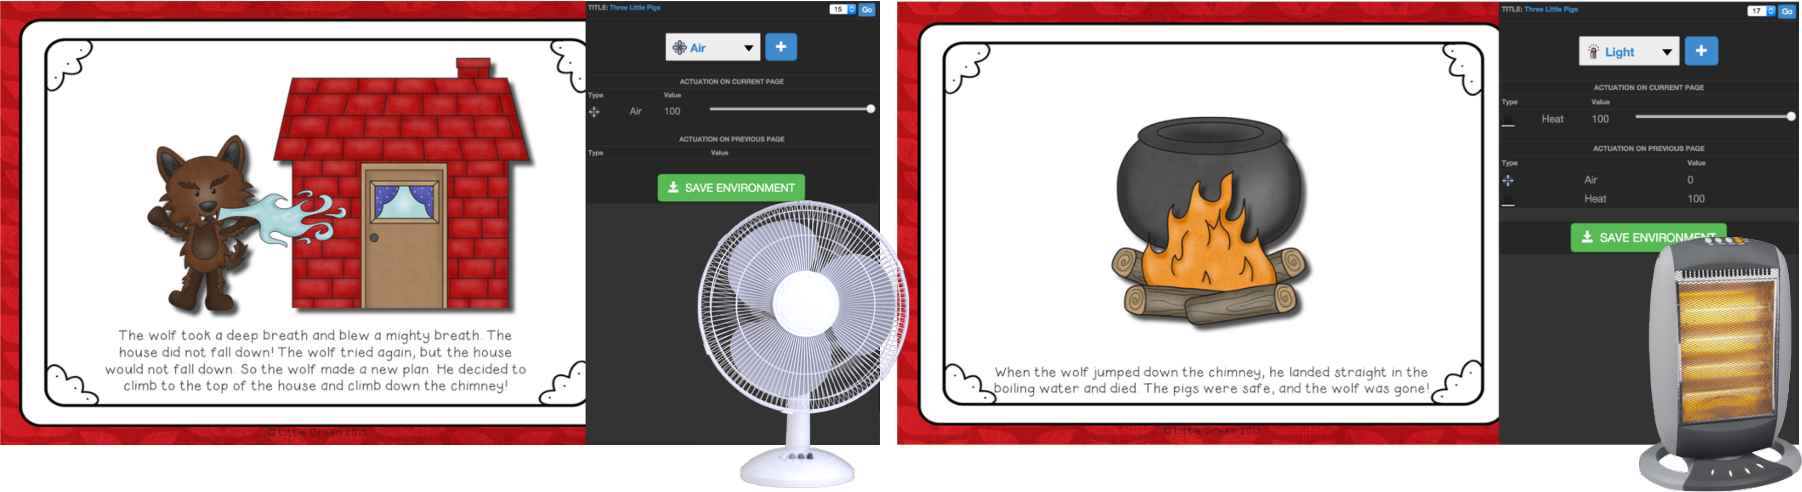
\includegraphics[width=\linewidth]{figures/teaser.pdf}
      \caption{Example story pages augmented with \name. (a) As the Big Bad Wolf huffs and puffs, a connected fan is triggered in the environment. (b) When the situation comes to a boil, a nearby heater warms the room. }
\label{fig:teaser}
\vspace{-8pt}
}
 
\maketitle

\begin{abstract}
Reading stories and experiencing storytelling is formative to a child's development and critical tool for sense-making. As the Internet of Things develops, we see new opportunities to expand the aesthetics of storytelling. We introduce SmartStorybook, an augmented environment (AE) application that controls the rich multimodal environment enabled by IoT to create interactive engagement with reading material. 
Smart Storybook contributes a content creation tool that synthesizes output with storylines. Upon reading time, the tool polls devices in a room for story enhancing capabilities (e.g. providing light, sound, smell). The desired story telling environment is resolved dynamically, providing a unique storytelling experience based on available devices and services.  
\end{abstract}


\keywords{
  internet of things, storytelling
}

\category{H.5.m.}{Information Interfaces and Presentation (e.g. HCI)}{Miscellaneous}
% \category{D.2.2}{Design Tools and Techniques}{User interfaces (H.5.2, H.1.2, I.3.6)}



%%%%%%%%%%%%%%%%%%%%%%%%%%%%%%%%%%%%%%%%%%
%%%%%%%%%%%%%%%% INTRODUCTION %%%%%%%%%%%%
%%%%%%%%%%%%%%%%%%%%%%%%%%%%%%%%%%%%%%%%%%
\newpage
\section{INTRODUCTION}
As reading technologies continue to develop, we have a new opportunity to alter and enhance the story telling experience. Story telling is fundamental to modern culture, as a means of passing knowledge and as a tool for sense-making. Interactive stories (the content) and interactive story books (the object) have been a long sought goal for human-computer interaction researchers in order to realize a long-term engagement and critical thinking. Due to the wide variety of publication mediums (print, digital, verbal) and a tension between traditional storytelling modalities, this has proved difficult. In particular, the spectacle of an augmented story book often overpowers the content and affects the learning value of the story itself. 

We present \name, a digital storybook that polls for IoT-connected devices and triggers actions based on story content. Our approach enhances the physical environment rather than imposing a virtual one. We show how this type of interface provides a seamless interaction with the storytelling experience and present novel application scenarios for improving sense-making and creating a dynamic story telling experience for repeat engagement with stories. 
   
%%%%%%%%%%%%%%%%%%%%%%%%%%%%%%%%%%%%%%%%%%
%%%%%%%%%%%%%%%% BACKGROUND %%%%%%%%%%%%%%
%%%%%%%%%%%%%%%%%%%%%%%%%%%%%%%%%%%%%%%%%%


  \begin{figure*}[th!]
      % \vspace{-8pt}
      \centering
      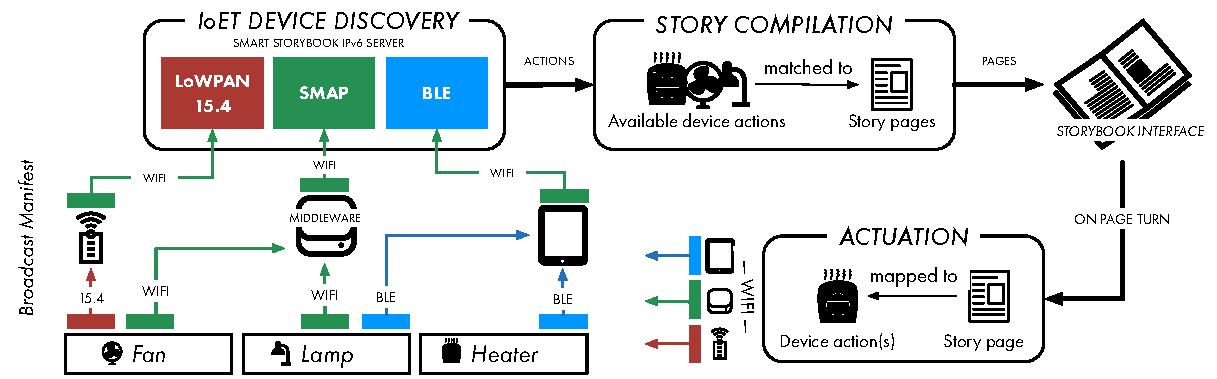
\includegraphics[keepaspectratio, width=0.98\textwidth]{figures/architecture.pdf} 
      \caption{\namesp architecture. Devices in a room broadcast available services through supported physical communication (Bluetooth, IEEE 802.15.4) in a IoET device discovery phase. A device-action list is then matched to desired actions in a story page. This story is pulled down by a storybook interface which publishes its page location. On a page turn event, the bound actions are actuated via its appropriately. }
      \vspace{-4pt}
      \label{fig:architecture} 
    \end{figure*}

\section{BACKGROUND}
The ``magic book'' has been long sought goal for interaction researchers.
Billinghurst, et al., proposes three spheres of interaction: the tangible object, the mixed-reality universe, and the virtual universe \cite{billinghurst_magicbook-moving_2001}. Several technologies have been used to operate in each of these spaces: refined computer vision techniques have been used to prove the feasibility of an augmented reality storybook free of machine-readable markup \cite{scherrer_haunted_2008}. Camera free approaches, such as Fujinami's augmented book cover and bookmark, detect page flips and offer a more mobile detection routine \cite{fujinami_page-flipping_2009}. Head-mounted displays with a book as interface have been shown to create immersive visual environments \cite{saso_little_2003}. Unlike mixed-reality initiatives that augment physical artifacts with virtual elements, Smart Storybook uses the StoryBubbles iPad storybook application to interface with devices and directly alter the real representation of the environment.

Other research has focused on added new interactivity to story books. 
Through simple energy harvesting, Karagozler, et al., demonstrated that powered devices can be embedded directly onto the pages of a story book \cite{karagozler_paper_2013}. A rubbing action is used to generate charge to drive LEDs and power e-paper displays and enable dynamic animations and hidden messages. 
Multimodal output have been integrated into printed artifacts \cite{iggulden_printed_1999} seen primarily in greeting cards. 

The enhanced storybook has also been examined as a method of creating a more collaborative story telling experience and enhancing the learning value of these books. Raffle, et al., demonstrated how Internet-connected storybooks could be used to create a telepresent story-telling between children and distant relatives \cite{raffle_family_2010}. The character Elmo was used to facilitate the remote interaction; however this caused attention issues since children were more prone to engage with the digital cartoon. SmartStorybook has a similar ``WOW'' factor characteristic of many new media storybooks, however we show how this is not merely a superficial element, but can be designed so children directly engage with the story content. 


%%%%%%%%%%%%%%%%%%%%%%%%%%%%%%%%%%%%%%%%%%
%%%%%%%%%%%%%%%% DESIGN  %%%%%%%%%%%%%%%%%
%%%%%%%%%%%%%%%%%%%%%%%%%%%%%%%%%%%%%%%%%%


\section{SYSTEM DESIGN}
Our architecture is composed of three major components - IoT devices (SVCD, BLE, 15.4), a middleware application used as a book repository and for content creation, and a previously developed iPad application (StoryBubbles) for viewing story content. The system architecture is depicted in Figure \ref{fig:architecture} and consists of three steps: discovery devices and services, mapping services to pages in a storybook, and actuating the necessary device through the appropriate protocol. 

\subsection{IoET Device Discovery} 
Several protocols exist for discovering devices in an environment. To allow for interoperability, we created a central repository that stores manifests for 15.4\footnote{802.15.4 6LoWPAN - Low power Wireless Personal Area Networks - a IPv6 protocol that enables small devices to have Internet-connectivity},
Bluetooth\footnote{Bluetooth Generic Attribute Profile},
and sMAP\footnote{The Simple Measurement and Actuation Profile (sMAP) is a specification for transmitting physical data to and from sensors and actuators \cite{dawson-haggerty_smap:_2010}.} 
devices. 

In this paper, we focus primarily on the actuation component of sMAP, which provides a specification for commonly used actuation patterns: binary two-state, discrete n-state, any-integer, and continuous-value actuation. A sMAP registered connected device publishes its available services to a middleware server and subscribes to a socket and listens for incoming requests. The server provides a RESTful HTTP API to get/set actuator state, while offering some rate-limiting control. 

This sMAP pattern was extended to devices published through 15.4 and Bluetooth. 
Metadata was added to published manifest for each device describing each action and its corresponding modality. 
Modality is described in terms of physical and sensory characteristics as follows: \quoted{$\langle$ light, air, sound, smell, heat, taste, motion $\rangle$}.
Each action was ascribed an amplitude (\quoted{on} $\rightarrow$ 100), and for locality a distance attribute was added to each environment. Lastly, a RESTful API set/get point was allocated to each device.

\subsection{Story compilation}
In order to allow story developers to author interactive content into existing storybooks, we created a IoT story composer that assigns a high-level description of a desired environment to a story page (Figure \ref{fig:composer}). For each page, a story developer can specify the intensity of each modality along a continuous range from 0 to 100. For usability, active actuations (triggered from previous pages) are displayed alongside the desired environment.

\subsubsection{Matching}
Two matching schemes where devices for resolving devices to desired environmental or interactive conditions. 
\begin{itemize}
\item Least-squares - takes the difference in desired environment and the permutation of IoT device actions and finds the closest optimal fit. 
\item Greedy - Finds the closest modality strength value and actuate $n$ equivalent actions (e.g. $\langle$\quoted{light}, 100, $n \rangle \rightarrow$ turn on $n$ \quoted{light} actuators). 

\end{itemize}
\subsection{Actuation}
The iPad storybook application pulls down storybook information from a server. Each page turn then functions as a button press. The server subscribes to this stream, and looks up appropriate devices to actuate. 
The server communicates with each protocol using a base station to handle actuation. For instance, BL devices are actuated using an iPad or other BL device as a relay. All device actuation logic exists in the middleware layer. 

 


\section{EXAMPLE STORY}
In a mock IoET storytelling environment, our system architecture discovered up to seven connected devices in the 19-page story of The Three Little Pigs by Little Green. The devices included a 4-state sMAP/15.4/BL fan and a sMAP smart powerstrip with binary control to 6 devices: 3 lights, a personal heater and fan, and a scent diffuser.  
  \begin{figure}[t!]
      % \vspace{-8pt}
      \centering
      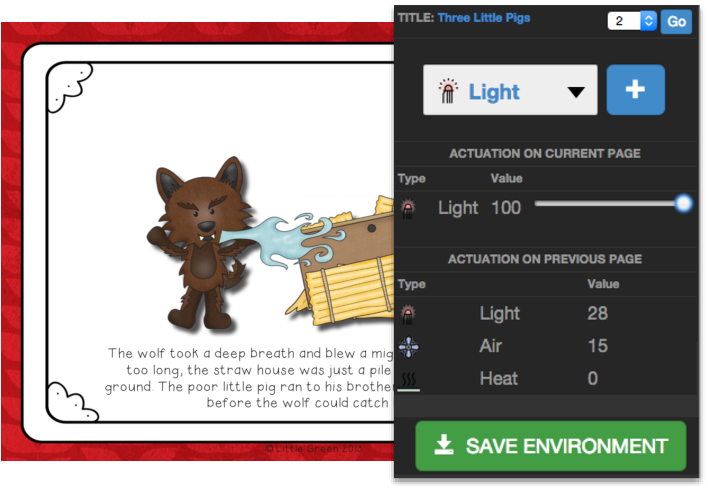
\includegraphics[keepaspectratio, width=0.5\textwidth]{figures/composer.pdf} 
      \caption{\namesp composer. Modalities are assigned to each page in the storybook to create a desired ambiance. Active page actuations are displayed to remind content authors of current conditions.}
      \vspace{-4pt}
      \label{fig:composer} 
    \end{figure}


%%%%%%%%%%%%%%%%%%%%%%%%%%%%%%%%%%%%%%%%%%
%%%%%%%%%%%%%%%% EVALUATION %%%%%%%%%%%%%%
%%%%%%%%%%%%%%%%%%%%%%%%%%%%%%%%%%%%%%%%%%

\section{APPLICATIONS}
\subsection{Augmented Environments}
Beyond visual animations that are present in screen-based applications, Smart Storybook interacts with a wider range of sensory experiences. By connecting to smart fans, Smart Storybook can control air flow. This allows us to simulate a cooler narrative.
\subsection{Character Enhancement}
Through, Smart Storybook's content creation tool, character actions are joined with environment coordinations. The reader experiences the actions of a character through various modalities. In our favorite example, the wolf in the Three Little Pigs blows down the house alongside a fan turned to high speed. These cues add theatricality as the story and environment become melded together, and signal to young readers character presence. 
\subsection{Dynamic Storytelling and Interactivity}
At each environment, Smart Storybook queries to find what devices are available to contribute to the storytelling experience. This means that each room has its own storytelling capabilities, and the story becomes anew with a new environment. For instance, the story Goodnight Moon, where a reader bids goodnight to the inhabitants of a room, can be made interactive such that each “good night” turns off an IoT device. By retaining the novelty of stories through different augmented environments, Smart Storybook can facilitate continued engagement with readers. 

%%%%%%%%%%%%%%%%%%%%%%%%%%%%%%%%%%%%%%%%%%%%%%%
%%%%%%%%   LIMITATIONS & FUTURE WORK  %%%%%%%%%
%%%%%%%%%%%%%%%%%%%%%%%%%%%%%%%%%%%%%%%%%%%%%%%

\section{LIMITATIONS AND FUTURE WORK}
Adding device metadata such as proximity and context information. Many devices are proxies for actions. The granularity of their service is suspect. This can be mediated through a user selection process. 
Richer actuator control is limited by connectivity. For instance, a lightning behavior (a lamp turning on and off rapidly) is subject to the throughput of the server.
Privacy and control. During the demo, several groups were using similar devices.A similar case would likely occur in the wild; access control needs to be added to devices to prevent unwanted behavior (such as acuating a thermometer of a building). 
%%%%%%%%%%%%%%%%%%%%%%%%%%%%%%%%%%%%%%%%%%%%%%%
%%%%%%%%%%%%%%%   CONCLUSION    %%%%%%%%%%%%%%%
%%%%%%%%%%%%%%%%%%%%%%%%%%%%%%%%%%%%%%%%%%%%%%%

\section{CONCLUSION}
Smart Storybook provides an alternative viewpoint to the IoT narrative. By project touches on issues of discovery management and ensemble creation. Ultimately, ascribing relevant metadata remains the chief deterrent to widespread applicability. While the sMAP definition provides some flexibility,  there is inherently a lack of proximity information and the granularity needed for storytelling. SVCD can provide better proximity data through RSSI, or resolving devices can be made a user-process.

%%%%%%%%%%%%%%%%%%%%%%%%%%%%%%%%%%%%%%%%%%
%%%%%%%%%%%%%%%% ACK %%%%%%%%%%%%%%%%%%%%%
%%%%%%%%%%%%%%%%%%%%%%%%%%%%%%%%%%%%%%%%%%

\section{ACKNOWLEDGEMENTS}
This work was done as a CS294 class project taught by Prof. David Culler. 
Team consisted of Aparna Dhinakaran, Michael Ho, Romi Phadte. 
The iPad Storybook application was used with permission from X. 

\balance
\bibliographystyle{acm-sigchi}
\bibliography{story}
\end{document}


